\documentclass[12pt]{standalone}
\usepackage[utf8]{inputenc}
\usepackage[T1]{fontenc}
\usepackage{times}
\usepackage{amsmath,amssymb}
\usepackage[dvipsnames,svgnames]{xcolor}
\usepackage{tikz}
\usetikzlibrary{calc, positioning, arrows.meta, decorations.pathreplacing}
\definecolor{dmrsfill}{HTML}{CDE2FB}
\definecolor{winblue}{HTML}{0D366B}
\definecolor{inksec}{HTML}{52514E}
\definecolor{interf}{HTML}{C0504D}
% R_n (M x M) em C x C blocos, exemplo com M = 12, C = 4 e M_c = 3. Cada célula é um par de
%     antenas (a, b). Os blocos da diagonal são estimados na DU (Zhao et al. 2025, Fig. 3); em
%     vermelho, os blocos da coluna 3, que a DU 3 usa (figura du_recebe).
\begin{document}
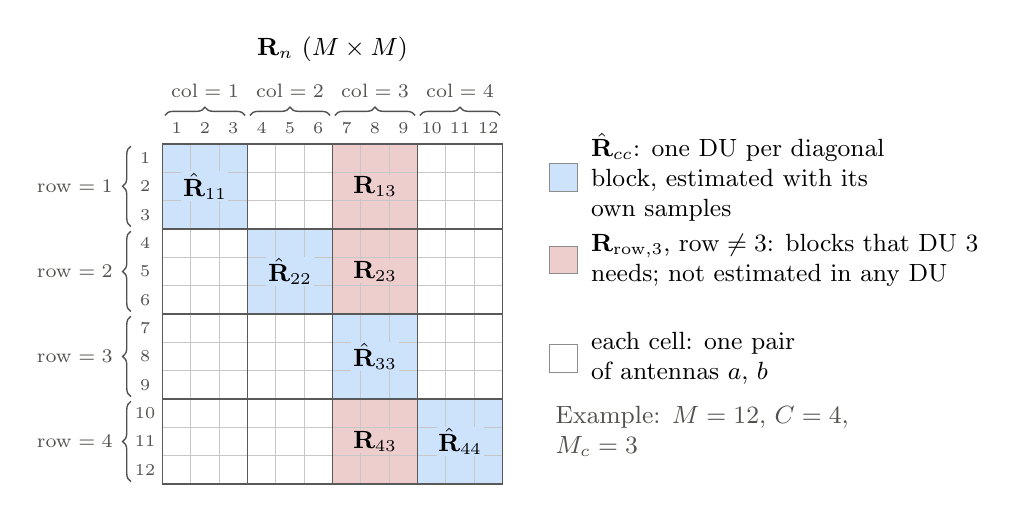
\begin{tikzpicture}[font=\fontsize{9}{10.8}\selectfont, >={Stealth[length=5pt]}]
\def\u{0.36}
\begin{scope}[shift={(0,0)}]
  % blocos coloridos
  \foreach \r in {0,...,3} \fill[dmrsfill] (3*\r*\u,-3*\r*\u) rectangle ++(3*\u,-3*\u);
  \fill[interf!28] (6*\u,0) rectangle ++(3*\u,-3*\u);
  \fill[interf!28] (6*\u,-3*\u) rectangle ++(3*\u,-3*\u);
  \fill[interf!28] (6*\u,-9*\u) rectangle ++(3*\u,-3*\u);
  % grade de M x M células (uma por par de antenas)
  \foreach \k in {0,...,12} {
    \draw[black!22, line width=0.3pt] (\k*\u,0) -- (\k*\u,-12*\u);
    \draw[black!22, line width=0.3pt] (0,-\k*\u) -- (12*\u,-\k*\u);
  }
  % divisão em blocos de M_c x M_c
  \foreach \k in {0,3,6,9,12} {
    \draw[black!65, line width=0.6pt] (\k*\u,0) -- (\k*\u,-12*\u);
    \draw[black!65, line width=0.6pt] (0,-\k*\u) -- (12*\u,-\k*\u);
  }
  % rótulos dos blocos
  \foreach \r in {1,...,4}
    \node[fill=dmrsfill, inner sep=0.6pt] at (3*\r*\u-1.5*\u,-3*\r*\u+1.5*\u) {$\hat{\mathbf R}_{\r\r}$};
  \node[fill=interf!28, inner sep=0.6pt] at (7.5*\u,-1.5*\u) {$\mathbf R_{13}$};
  \node[fill=interf!28, inner sep=0.6pt] at (7.5*\u,-4.5*\u) {$\mathbf R_{23}$};
  \node[fill=interf!28, inner sep=0.6pt] at (7.5*\u,-10.5*\u) {$\mathbf R_{43}$};
  % índices das antenas
  \foreach \k in {1,...,12} {
    \node[inksec, font=\fontsize{6}{7}\selectfont] at (\k*\u-\u/2,0.2) {\k};
    \node[inksec, font=\fontsize{6}{7}\selectfont] at (-0.22,-\k*\u+\u/2) {\k};
  }
  % clusters
  \foreach \c in {1,...,4} {
    \draw[decorate, decoration={brace, amplitude=3pt}, inksec, line width=0.5pt] (3*\c*\u-3*\u+0.03,0.36) -- (3*\c*\u-0.03,0.36) node[midway, above=3pt, font=\fontsize{7.5}{9}\selectfont] {$\mathrm{col} = \c$};
    \draw[decorate, decoration={brace, amplitude=3pt, mirror}, inksec, line width=0.5pt] (-0.4,-3*\c*\u+3*\u-0.03) -- (-0.4,-3*\c*\u+0.03) node[midway, left=3pt, font=\fontsize{7.5}{9}\selectfont] {$\mathrm{row} = \c$};
  }
  \node at (6*\u,1.2) {$\mathbf R_n$ ($M \times M$)};
  % legenda
  \def\lx{12*\u+0.6}
  \fill[dmrsfill] (\lx,-0.25) rectangle ++(0.35,-0.35);
  \draw[black!45, line width=0.4pt] (\lx,-0.25) rectangle ++(0.35,-0.35);
  \node[right, align=left] at (\lx+0.4,-0.425) {$\hat{\mathbf R}_{cc}$: one DU per diagonal\\block, estimated with its\\own samples};
  \fill[interf!28] (\lx,-1.3) rectangle ++(0.35,-0.35);
  \draw[black!45, line width=0.4pt] (\lx,-1.3) rectangle ++(0.35,-0.35);
  \node[right, align=left] at (\lx+0.4,-1.475) {$\mathbf R_{\mathrm{row},3}$, $\mathrm{row} \neq 3$: blocks that DU 3\\needs; not estimated in any DU};
  \draw[black!45, line width=0.4pt] (\lx,-2.55) rectangle ++(0.35,-0.35);
  \node[right, align=left] at (\lx+0.4,-2.725) {each cell: one pair\\of antennas $a$, $b$};
  \node[right, align=left, inksec] at (\lx-0.05,-3.65) {Example: $M = 12$, $C = 4$,\\$M_c = 3$};
\end{scope}
\end{tikzpicture}
\end{document}
